\documentclass{beamer}
%
% Choose how your presentation looks.
%
% For more themes, color themes and font themes, see:
% http://deic.uab.es/~iblanes/beamer_gallery/index_by_theme.html
%
\mode<presentation>
{
  \usetheme{Madrid}      % or try Darmstadt, Madrid, Warsaw, ...
  \usecolortheme{beaver} % or try albatross, beaver, crane, ...
  \usefonttheme{serif}  % or try serif, structurebold, ...
  \setbeamertemplate{navigation symbols}{}
  \setbeamertemplate{caption}[numbered]
} 

\usepackage[english]{babel}
\usepackage{kotex}
\usepackage{tikz}
%\usepackage[utf8x]{inputenc}
\usepackage{listings}
\usepackage{amsfonts}
\usepackage[linesnumbered,ruled,vlined]{algorithm2e}
\usepackage{algorithmic}

% algorithmbis environment
\makeatletter
\newcounter{algorithmbis}[section]
\setcounter{algorithmbis}{0}
\renewcommand{\thealgorithmbis}{\arabic{algorithmbis}}
\def\algorithmbis{\@ifnextchar[{\@algorithmbisa}{\@algorithmbisb}}
\def\@algorithmbisa[#1]{%
  \refstepcounter{algorithmbis}
  \trivlist
  \leftmargin\z@
  \itemindent\z@
  \labelsep\z@
  \item[\colorbox{lightgray}{\parbox{\textwidth}{%
	    \noindent\strut\textbf{\sf\small 코드 \sf\small\thealgorithmbis} \sf\small#1}
  }]\hfil\vskip0em%
  \color{darkgray}
}
\def\@algorithmbisb{\@algorithmbisa[]}
\def\endalgorithmbis{\hfil\endtrivlist}
\makeatother

\lstset{ %
  backgroundcolor=\color{white},   % choose the background color; you must add \usepackage{color} or \usepackage{xcolor}
  basicstyle=\footnotesize,        % the size of the fonts that are used for the code
  breakatwhitespace=false,         % sets if automatic breaks should only happen at whitespace
  breaklines=true,                 % sets automatic line breaking
  captionpos=b,                    % sets the caption-position to bottom
  commentstyle=\color{gray},    % comment style
  deletekeywords={...},            % if you want to delete keywords from the given language
  escapeinside={\%*}{*)},          % if you want to add LaTeX within your code
  extendedchars=true,              % lets you use non-ASCII characters; for 8-bits encodings only, does not work with UTF-8
  frame=single,                    % adds a frame around the code
  keepspaces=true,                 % keeps spaces in text, useful for keeping indentation of code (possibly needs columns=flexible)
  keywordstyle=\color{blue},       % keyword style
  language=C++,                 % the language of the code
  morekeywords={*,...},            % if you want to add more keywords to the set
  numbers=left,                    % where to put the line-numbers; possible values are (none, left, right)
  numbersep=5pt,                   % how far the line-numbers are from the code
  numberstyle=\tiny\color{gray}, % the style that is used for the line-numbers
  rulecolor=\color{black},         % if not set, the frame-color may be changed on line-breaks within not-black text (e.g. comments (green here))
  showspaces=false,                % show spaces everywhere adding particular underscores; it overrides 'showstringspaces'
  showstringspaces=false,          % underline spaces within strings only
  showtabs=false,                  % show tabs within strings adding particular underscores
  stepnumber=1,                    % the step between two line-numbers. If it's 1, each line will be numbered
  stringstyle=\color{gray},     % string literal style
  tabsize=2,                       % sets default tabsize to 2 spaces
  title=\lstname                   % show the filename of files included with \lstinputlisting; also try caption instead of title
}

\title[3D 그래픽스 프로그래밍]{그래픽스 강의노트 03 - OpenGL 소개 (일부)}
\author{강영민}
\institute{동명대학교}
\date{2015년 2학기}

\begin{document}

%%%%%%%%%%%%%%%%%%%%%%%%%%%%%%%%%%%%%%%%%%%%%%%%%%%%%%%%%
\begin{frame}
  \titlepage
\end{frame}

% Uncomment these lines for an automatically generated outline.
%\begin{frame}{Outline}
%  \tableofcontents
%\end{frame}


%%%%%%%%%%%%%%%%%%%%%%%%%%%%%%%%%%%%%%%%%%%%%%%%%%%%%%%%%
\begin{frame}{OpenGL}

\begin{itemize}
\item OpenGL은 특정한 하드웨어나 운영체제에 의존하지 않고 다양한 시스템에 이식(移植)될 수 있는 개방형 라이브러리
\item OpenGL을 통한 학습은 실시간 그래픽스에 대한 이해를 돕고, 다양한 시스템에 적용가능한 그래픽스 프로그래밍 기술을 습득하게 함
\end{itemize}
\end{frame}
%%%%%%%%%%%%%%%%%%%%%%%%%%%%%%%%%%%%%%%%%%%%%%%%%%%%%%%%%

%%%%%%%%%%%%%%%%%%%%%%%%%%%%%%%%%%%%%%%%%%%%%%%%%%%%%%%%%
\begin{frame}{OpenGL을 사용하기 위한 준비}

\begin{itemize}
\item Mac OS X, Linux - 특별한 준비가 필요 없음
\item MS Windows - 플랫폼 독립적 윈도우 생성을 위해 glut를 따로 설치해야 함
\end{itemize}

\begin{itemize}
\item 수업에 사용할 glut 라이브러리
	\begin{itemize}
	\item freeglut
	\item 다운로드 - precompiled binary는 64비트 
	\item 32비트와 64비트 용으로 컴파일한 결과를 수업 홈페이지에 게시
	\end{itemize}
\end{itemize}

\end{frame}
%%%%%%%%%%%%%%%%%%%%%%%%%%%%%%%%%%%%%%%%%%%%%%%%%%%%%%%%%


%%%%%%%%%%%%%%%%%%%%%%%%%%%%%%%%%%%%%%%%%%%%%%%%%%%%%%%%%
\begin{frame}{MS Windows 환경에서 freeglut 설치}

\begin{itemize}
\item 32비트
	\begin{itemize}
	\item freeglutd.dll, freeglut.dll $\rightarrow$ C:$\backslash$System32
	\item 헤더 파일들 $\rightarrow$ (Windows SDK)$\backslash$include$\backslash$GL
	\item 라이브러리 파일들 (freeglutd.lib, freeglut.lib) $\rightarrow$ (Windows SDK)$\backslash$lib
	\end{itemize}
\end{itemize}

\begin{itemize}
\item 64비트
	\begin{itemize}
	\item freeglutd.dll, freeglut.dll $\rightarrow$ C:$\backslash$SystemWOW
	\item 헤더 파일들 $\rightarrow$ (Windows SDK)$\backslash$include$\backslash$GL
	\item 라이브러리 파일들 (freeglutd.lib, freeglut.lib) $\rightarrow$ (Windows SDK)$\backslash$lib$\backslash$l64
	\end{itemize}
\item 프로젝트의 플랫폼을 Win32가 아니라 64비트로 변경하여 생성하여야 함
\end{itemize}

\end{frame}
%%%%%%%%%%%%%%%%%%%%%%%%%%%%%%%%%%%%%%%%%%%%%%%%%%%%%%%%%


\begin{algorithmbis}[간단한 OpenGL 프로그램의 예]\label{code:OGL_opengl:example}
\lstset{language=C++, escapechar=^} 
\begin{lstlisting}

#ifdef WIN32 // window 
#include <windows.h>
#include <gl/gl.h>
#include <gl/glut.h>
#else // mac
#include <OpenGL/OpenGL.h>
#include <GLUT/GLUT.h>
#endif

void myDisplay() {
    glClear(GL_COLOR_BUFFER_BIT);
    glFlush();    
}

int main (int argc, char * argv[]) {
    glutInit(&argc, argv);
    glutInitDisplayMode(GLUT_SINGLE|GLUT_RGBA);
    glutInitWindowPosition(0, 0);
    glutInitWindowSize(512, 512);
    glutCreateWindow("A Triangle");  // ^{\it 윈도우 생성}^

    glClearColor(1.0, 0.0, 0.0, 1.0);
    glutDisplayFunc(myDisplay);	// ^{\it 디스플레이 콜백 등록}^
    glutMainLoop();				// ^{\it 이벤트 루프로}^

    return 0;
}
\end{lstlisting}
\end{algorithmbis}

%%%%%%%%%%%%%%%%%%%%%%%%%%%%%%%%%%%%%%%%%%%%%%%%%%%%%%%%%

\end{document}



\section{OpenGL 소개와 간단한 프로그래밍}

OpenGL은 개방형 그래픽스 라이브러리(Open Graphics Library)이다. 개방형이라는 것은 이 라이브러리의 소스 코드가 공개되어 있으며, 무료로 배포되며, 플랫폼(platform)에 독립적이라는 의미이다. 이 그래픽 라이브러리는 영화나 애니메이션 등에서 사용되는 고품질 오프라인 렌더링(rendering)을 위한 것이 아니라 게임이나 가상현실과 같이 실시간 렌더링을 위해 주로 사용된다. 따라서 이 라이브러리의 특징은 근사(approximation)을 통한 빠른 렌더링이다. 그래픽 하드웨어의 비약적인 발전에 따라 OpenGL을 통한 렌더링 결과의 품질 역시 매우 높은 수준에 도달하고 있지만, 근본적으로 오프라인 렌더링과는 다른 접근법을 사용하고 있다. 대표적인 예가 오프라인 렌더링은 전역 조명(global illumination)을 사용하여 빛이 표면에 반사되고 움직이는 것을 추적하여 여러 물체를 밝게 만드는 것이 가능하다는 것이다. 반면, 특별한 기법을 사용하지 않은 일반적인 OpenGL 렌더링 결과는 지역 조명(local illumination) 모델을 사용한다. 이 모델에서는 기하 객체가 다른 기하 객체는 고려하지 않고 오로지 빛과 자신 사이의 관계만을 고려하여 음영을 결정한다. 

\subsection{OpenGL의 특징}
OpenGL은 실시간 그래픽 라이브러리로서 사실상의 산업 표준이다. 이 라이브러리는 개방형이므로 플랫폼에 독립적이라는 중요한 특성을 가진다. 따라서 OpenGL을 이용하여 작성한 그래픽 프로그램은 여러 종류의 다른 운영체제를 가진 시스템에 쉽게 이식될 수 있다.

\index{상태 기계}\index{state machine}
OpenGL은 상태 기계(state machine)이다. 이것은 OpenGL의 동작이 현재의 상태에 의해 결정되며, 이 상태는 변경하지 않으면 계속해서 유지된다는 것이다.
OpenGL에는 많은 종류의 상태 변수가 있으며, 이 상태는 한 번 설정하면 다시 변경하지 않는 한 계속해서 설정된 상태를 유지하게 된다.
다시 말해, 선의 두께를 결정했다면, 이후에 이 두께를 변경하지 않는 이상 모든 선이 설정된 두께로 그려지게 된다.

\subsection{OpenGL 관례(convention)}

\index{OpenGL!관례}
OpenGL API의 명령들은 gl-Command-dimension-type의 꼴을 가진다. 예를 들어 glVertex3f는 정점(Vertex)의 위치를 설정하는 OpenGL 명령으로 3차원 데이터이며, 각 차원의 값을 부동소수점(floating point)로 표현한다는 의미가 된다.
OpenGL 명령어의 뒤에 붙어 입력 파라미터의 자료형을 표시하는 접미사는 표. \ref{tab:OGL_opengl:convention}과 같다.

\index{GLUT}
OpenGL을 사용할 때는 그래픽 장치를 다루는 핵심적 명령들로 구성된 OpenGL 라이브러리와 함께 카메라 등을 다루는 OpenGL 유틸리티 라이브러리를 함께 사용하는데, 유틸리티 라이브러리의 명령들은 glu로 시작한다. 또한 다양한 시스템의 서로 다른 윈도 환경에 독립적인 프로그램을 하기 위해 윈도 관리를 지원하는 OpenGL 유틸리티 툴킷 (utility toolkit)을 사용하는데, 이 툴킷의 명령들은 glut로 시작한다.


\begin{table}
\begin{tabular}{|c|l|l|l|} \hline
f & 32 비트 부동소수점 & float & GLfloat \\ \hline
d & 64 비트 부동소수점 & double & GLdouble \\ \hline
b & 8 비트 정수 & char & GLbyte \\ \hline
ub & 8 비트 부호 없는 정수 & unsigned char & GLubyte \\ \hline
i & 32 비트 정수 & int or long & GLint \\ \hline
ui & 32 비트 부호 없는 정수  & unsigned int 혹은 unsigned long & GLuint, GLenum \\ \hline
s & 16 비트 정수 & short & GLshort \\ \hline
\end{tabular}
\caption{OpenGL 명령어의 접미사 관례}
\label{tab:OGL_opengl:convention}
\end{table}
\subsection{OpenGL 프로그래밍 구조}

가장 간단한 OpenGL 프로그램은 코드. \ref{code:OGL_opengl:framework}와 같은 방식으로 이루어진다.
이 의사코드(pseudocode)를 살펴 보자. 우선 OpenGL을 사용하는 데에 필요한 헤더 파일 등을 포함한다.
그리고 두 개의 함수가 있는데, 먼저 나타난 함수는 화면 그리기를 수행하는 디스플레이(display) 콜백(callback)이며,
그 다음은 프로그램의 진입 지점인 메인(main) 함수이다.

OpenGL 프로그램은 윈도우를 띄우고, 이벤트가 발생할 때마다 해당 이벤트를 처리하는
이벤트 기반 프로그램(event-driven program)이다.
여러 가지 이벤트 처리 함수를 사용하는데, 가장 중요한 이벤트 처리 동작은 화면 그리기 이벤트를 처리하는
디스플레이 콜백이다. 
화면을 그려내는 작업은 그려야할 대상에 대해 적절한 변환을 설정하고, 
그리기에 사용할 프리미티브(primitive)를 설정한 뒤에 정점 데이터를 제공하는 방식이다.
프리미티브에 대해서는 다시 설명할 것이다.

메인 함수가 하는 일은 윈도우를 생성하고 초기화하는 일,
그리고 카메라의 투영 속성을 설정하고, 위치를 잡는 일을 한 뒤에
이벤트를 처리할 콜백을 등록하는 작업이다.
이런 작업들이 마무리되면 이벤트를 기다리는 루프(loop)로 들어간다.

\begin{algorithmbis}[OpenGL 프로그래밍의 기본 구조]\label{code:OGL_opengl:framework}
\lstset{language=C++, , escapechar=^} 
\begin{lstlisting}
#include <whateveryouwant> 

callback_fnc_for_display() {
   for(^{\sf 그려질 모든 객체에 대해^) {
      ^{\it 변환 설정;}^
      glBegin(^{\sf 그리기 프리미티브 지정}^);
      	^{\sf [[정점(vertex) 정보 제공;]]}^
      glEnd(); 
   }
   glFlush() ^{\it 또는}^ glutSwapBuffers();
}

void main(int argc, char **argv) {

   ^{\sf [[윈도우 초기화;]]}^

   glMatrixMode(GL_PROJECTION); 
   ^{\sf [[투영 행렬 설정;]]}^
   glMatrixMode(GL_MODELVIEW); 
   ^{\sf [[카메라의 위치와 방향 잡기;]]}^

   ^{\sf [[콜백 함수의 등록;]]}^
   ^{\sf [[메인 루프로 들어가기;]]}^
}
\end{lstlisting}
\end{algorithmbis}


이제 실제로 동작하는 간단한 OpenGL 코드를 작성해 보자.
코드 \ref{code:OGL_opengl:example}는 삼각형을 그리는 간단한 OpenGL 프로그램이다. 
이 코드를 실행한 결과가 그림. \ref{fig:OGL_opengl:simpleEx}에 나타나 있다.
앞에서 본 의사코드와 같이 두 개의 함수로 구성되어 있으며,
디스플레이 콜백 함수의 이름은 {\sf myDisplay}이다.
코드 \ref{code:OGL_opengl:framework}와 비교하며 실제 동작하는 코드를 살펴 보라.
이 코드에서 디스플레이 콜백은 {\sf GL\_POLYGON}을 그리기 프리미티브로 사용하고 있으며,
삼각형을 그리기 위한 세 개의 정점 데이터가 제공되었다. 그리고 각각의 정점은 색상이 지정되어 있다.

\begin{algorithmbis}[간단한 OpenGL 프로그램의 예]\label{code:OGL_opengl:example}
\lstset{language=C++, escapechar=^} 
\begin{lstlisting}
#ifdef WIN32 // window 
#include <windows.h>
#include <gl/gl.h>
#include <gl/glut.h>
#else // mac
#include <OpenGL/OpenGL.h>
#include <GLUT/GLUT.h>
#endif

void myDisplay() {
    glClear(GL_COLOR_BUFFER_BIT);
    glBegin(GL_POLYGON);
    glColor3f(1.0, 0.0, 0.0);
    glVertex3f(0.0, 0.0, 0.0);
    glColor3f(0.0, 0.0, 1.0);
    glVertex3f(0.5, 0.0, 0.0);
    glColor3f(0.0, 1.0, 0.0);
    glVertex3f(0.0, 0.5, 0.0);
    glEnd();
    glFlush();    
}

int main (int argc, char * argv[]) {
    glutInit(&argc, argv);
    glutInitDisplayMode(GLUT_SINGLE|GLUT_RGBA);
    glutInitWindowPosition(0, 0);
    glutInitWindowSize(512, 512);
    glutCreateWindow("A Triangle");  // ^{\it 윈도우 생성}^
    glClearColor(1.0, 0.0, 0.0, 1.0);
    glutDisplayFunc(myDisplay);	// ^{\it 디스플레이 콜백 등록}^
    glutMainLoop();				// ^{\it 이벤트 루프로}^
    return 0;
}
\end{lstlisting}
\end{algorithmbis}




\begin{figure}[h!]
  \centering
    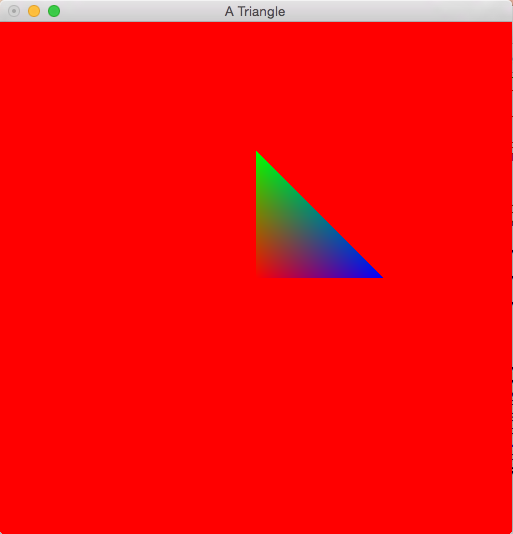
\includegraphics[height=8cm]{OGL_opengl/simpleEx.png}
    \caption{간단한 OpenGL 프로그램의 실행 결과}
    \label{fig:OGL_opengl:simpleEx}
\end{figure}


\section{프리미티브(primitive): 그리기 기본요소}

\index{OpenGL!primitives}\index{primitives}
\index{프리미티브}\index{그리기 기본요소}
OpenGL을 이용하여 그림을 그릴 때에 가장 중요한 것은 정점(vertex) 데이터를 설정하는 것이다. 이 정점 데이터는 그래픽 하드웨어로 넘겨지는데, 그래픽 하드웨어는 이 정점들을 몇 개 씩 묶어 하나의 그리기 대상으로 간주해야 하는지를 알아야 한다. 이 판단은 프로그래머(programmer)가 지정한 프리미티브(primitive) 설정에 따른다. 
프리미티브는 OpenGL이 제공하는 그리기 기본요소라고 할 수 있다.
예를 들어 프로그래머가 ‘점’이라는 기본요소를 선택했다면, 
그래픽 하드웨어는 이후의 모든 정점들을 하나씩 점으로 그리면 된다. 
그러나 만약 프로그래머가 ‘선분’이라는 요소를 선택했다고 하면, 그래픽 하드웨어는 입력되는 정점들을 두 개씩 묶어 각각 하나의 선분으로 표현해야 한다. 

입력 정점들을 어떻게 조합할 것인가를 결정하는 것이 그리기 기본요소, 혹은 프리미티브(primitive)라고 한다. OpenGL에서 사용가능한 그리기 기본요소를 알아보자.
OpenGL에서는 위의 그림과 같은 기본요소를 사용할 수 있다. 정점은 v0부터 숫자에 따라 차례대로 입력되었다고 가정한다. OpenGL 그리기의 기본은 이 기본요소를 이용하여 다음과 같은 코드. \ref{code:OGL_opengl:primitiveUsage}의 방식으로 정점을 넘겨주는 것이다.

\begin{algorithmbis}[그리기 기본요소를 사용하는 방법]\label{code:OGL_opengl:primitiveUsage}
\lstset{language=C++, escapechar=^} 
\begin{lstlisting}
glBegin(^{\sf drawing primitive}^);
      // vertex position, color, normal, etc
      setVertexInfo(); 
glEnd(); 
\end{lstlisting}
\end{algorithmbis}

OpenGL에서 기본요소의 이름은 ‘GL\_‘로 시작하며 다음과 같은 것들이 있다.

\begin{itemize}
\item {\sf GL\_POINTS}: 입력된 정점을 하나씩 점으로 가시화
\item {\sf GL\_LINES}: 입력된 정점을 두 개씩 묶어 선분으로 표현 
\item {\sf GL\_LINE\_STRIP}: 입력된 정점을 차례대로 연결하여 하나의 폴리라인(polyline)을 구성
\item {\sf GL\_LINE\_LOOP}: 입력된 정점을 차례로 연결한 뒤에 마지막 점을 시작점으로 연결
\item {\sf GL\_TRIANGLES}: 입력된 정점을 세 개씩 묶어 삼각형을 그림
\item {\sf GL\_TRIANGLE\_STRIP}: 처음 세 개 정점으로 삼각형을 그린 뒤, 정점이 추가될 때마다 삼각형을 직전 두 개 정점과 연결하여 삼각형 추가 
\item {\sf GL\_TRIANGLE\_FAN}: 부채 모양으로 삼각형을 추가해 나감
\item {\sf GL\_QUADS}: 정점 네 개씩을 묶어 사각형 그리기
\item {\sf GL\_QUAD\_STRIP}: 처음 네 개 정점으로 사각형 그리고, 이후 두 개씩 묵어 직전 두 개 정점과 함께 사각형 그리기
\item {\sf GL\_POLYGON}: 입력된 모든 정점으로 다각형을 그림
\end{itemize}

이러한 기본요소를 이용하여 그릴 수 있는 도형의 실제 예는 그림. \ref{fig:OGL_opengl:primitives}와 같다.

\begin{figure}[h!]
  \centering
    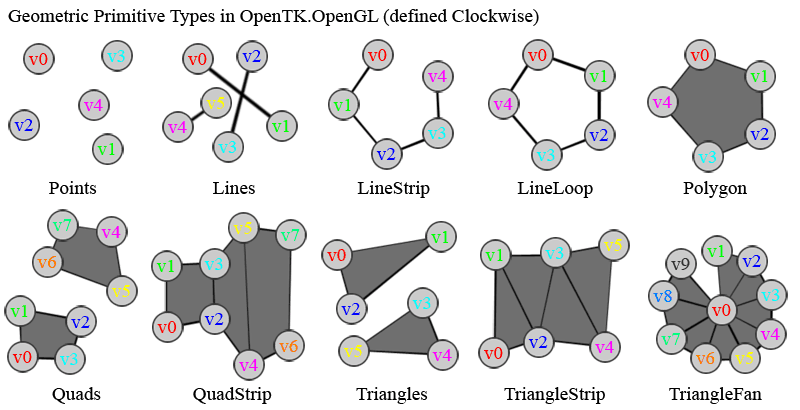
\includegraphics[height=7cm]{OGL_opengl/primitives.png}
    \caption{OpenGL 그리기 기본요소}
    \label{fig:OGL_opengl:primitives}
\end{figure}

정점 데이터는 위치와 법선벡터, 색 등을 설정할 수 있는데, 우선 정점의 위치만을 입력한다면 glVertex[dim-type]으로 입력한다. 예를 들어 3 차원 정점의 각 성분을 부동소수점 표현으로 넣는다면, glVertex3f(x,y,z)와 같이 입력할 수 있다. 그 외에도 다음 크드. \ref{code:OGL_opengl:verticessetting}과 같은 여러 표현이 가능하다.

\begin{algorithmbis}[정점 데이터 설정 방법]\label{code:OGL_opengl:verticessetting}
\lstset{language=C++} 
\begin{lstlisting}
float x,y,z;
double dx,dy,dz;
int ix,iy,iz;
float verts = {1.0f, 2.0f, 1.0f};
glBegin(drawing primitive);
      glVertex3f(x,y,z);
      glVertex3d(dx,dy,dz);
      glVertex3i(ix,iy,iz);
      glVertex3fv(verts);
glEnd();
\end{lstlisting}
\end{algorithmbis}

이러한 프리미티브를 이용하여 다양한 장면을 그려낼 수 있다. 앞서 살펴본 코드. \ref{code:OGL_opengl:example}의 
display 함수를 다음과 같이 수정하여 간단한 풍경을 그려볼 수 있다. 

\begin{algorithmbis}[다양한 프리미티브의 적용]\label{code:OGL_opengl:simpleScene}
\lstset{language=C++, escapechar=^} 
\begin{lstlisting}
...
#include <math.h>
void myDisplay() {
    glClear(GL_COLOR_BUFFER_BIT);
    // ^{\it 색상의 지정}^
    glColor3f(0.0, 1.0, 0.0);    

    // ^{\it 삼각형 그리기로 지정}^
    glBegin(GL_TRIANGLES);
    // mountain 1
    glVertex2f(-0.75, -0.25);
    glVertex2f(0.0, 0.25);
    glVertex2f(0.25, -0.25);
    // mountain 2 - ^{\it 그리기 색상 변경}^
    glColor3f(0.5, 0.5, 0.1);
    glVertex2f(-0.25, -0.25);
    glVertex2f(0.75, 0.25);
    glVertex2f(1.0, -0.25);
    glEnd();

    // ^{\it 사각형 그리기로 지정}^
    glBegin(GL_QUADS);
    // roof ^{\it 파란색으로 색상 변경}^
    glColor3f(0.0, 0.0, 1.0);
    glVertex2f(-1.0, 0.25);
    glVertex2f(-0.75, 0.5);
    glVertex2f(-0.25, 0.5);
    glVertex2f(0.0, 0.25);
    // house ^{\it 노란색으로 색상 변경}^
    glColor3f(1.0, 1.0, 0.0);
    glVertex2f(-0.75, 0.25);
    glVertex2f(-0.75, -0.25);
    glVertex2f(-0.25, -0.25);
    glVertex2f(-0.25, 0.25);
    // tree ^{\it 갈색으로 변경}^
    glColor3f(0.7, 0.5, 0.0);
    glVertex2f(0.5, 0.25);
    glVertex2f(0.75, 0.25);
    glVertex2f(0.75, -0.25);
    glVertex2f(0.5, -0.25);
    glEnd();

    // ^{\it 입력된 정점을 모두 이용하는 다각형 그리기로 지정}^
    glBegin(GL_POLYGON);
    int n=20;
    float radius=0.1;
    glColor3f(1.0, 1.0, 0.0);
    float angle = 0.0; float step=(3.14159*2.0)/n;
    // ^{\it 반복문 내에서 여러 개의 정점 좌표를 계산한 뒤에 지정하는 방식}^
    // ^{\it 여기서는 원을 이루는 정점들을 계산하고 있음}^
    while (angle<3.14159*2.0) {
        glVertex2f(radius*cos(angle), radius*sin(angle)+0.75);
        angle += step;
    }
    glEnd();

    // ^{\it 원의 중심을 옮기고 반지름을 바꾼 뒤에 다시 그림}^
    glBegin(GL_POLYGON);
    n=20;
    radius=0.25;
    glColor3f(0.0, 1.0, 0.0);
    angle = 0.0; step=(3.14159*2.0)/n;
    while (angle<3.14159*2.0) {
        glVertex2f(radius*cos(angle)+0.625, radius*sin(angle)+0.25);
        angle += step;
    } 
    glEnd();
    glFlush();
}
\end{lstlisting}
\end{algorithmbis}

이 프로그램을 실행한 결과는 그림 \ref{fig:OGL_opengl:simpleScene}에 나타나 있다.  삼각형 두 개로 산 모양을 만들었고,
갈색 사각형으로 나무의 줄기, 노란색 사각형으로 집의 벽, 파란색 사각형으로 지붕을 그렸다.
두 개의 원은 태양과 나뭇잎을 표현했다.

\begin{figure}[h!]
  \centering
    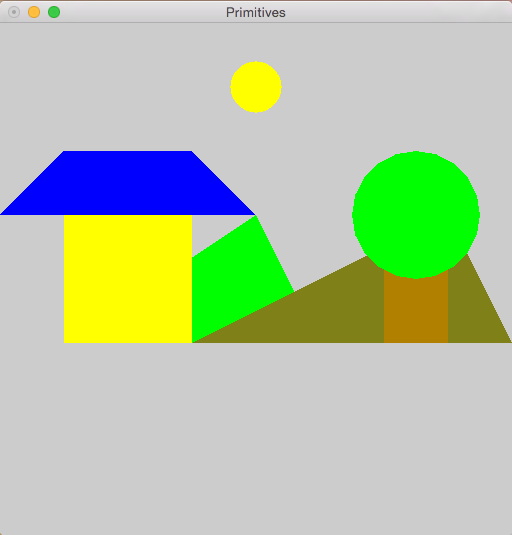
\includegraphics[height=10cm]{OGL_opengl/simpleScene.png}
    \caption{간단한 장면의 구현}
    \label{fig:OGL_opengl:simpleScene}
\end{figure}

\section{간단한 카메라 설정}

\index{camera}\index{카메라}
앞서 작성한 코드는 카메라에 대한 조작을 전혀 포함하지 않고 있다. 
이때 사용된 카메라는 디폴트(default) 카메라로서 원점에 놓여서 $z$ 축 음의 방향을 쳐다보는 카메라이다. 
이 디폴트 카메라는 원근을 고려하지 않는 카메라로서 객체의 위치가 $(x,y,z)$라면 이를 $(x,y,0)$으로 떨어뜨린다.
3차원 그래픽스를 하기 위해서는 3차원 공간을 자유롭게 움직이며 물체를 관찰할 수 있어야 하는데, 
이렇게 고정된 위치에서 제한적인 투영만 적용해서는 다양한 장면을 연출할 수 없다. 
카메라를 제어하는 관측과 관련해서는 다시 자세히 다룰 것이지만 
우선 간단히 투영에 대한 이해를 해보자.


\subsection{디폴트 카메라 (default camera)}

\index{디폴트 카메라}\index{default camera}
OpenGL의 디폴트 카메라는 원점에 놓여 있으며, z축 음의 방향을 쳐다본다. 원근 투영을 적용하지 않으며, 따라서 카메라에 잡히는 공간은 상자 형태가 된다. 실제 상자의 모양은 중심이 원점에 있고 각 변의 길이가 2이다. 이러한 원근이 없는 투영은 glOrtho를 통해 설정한다. 그림. \ref{fig:OGL_opengl:defaultCam}는 이러한 디폴트 카메라의 개념을 시각적으로 보이고 있다.

\begin{figure}[h!]
  \centering
    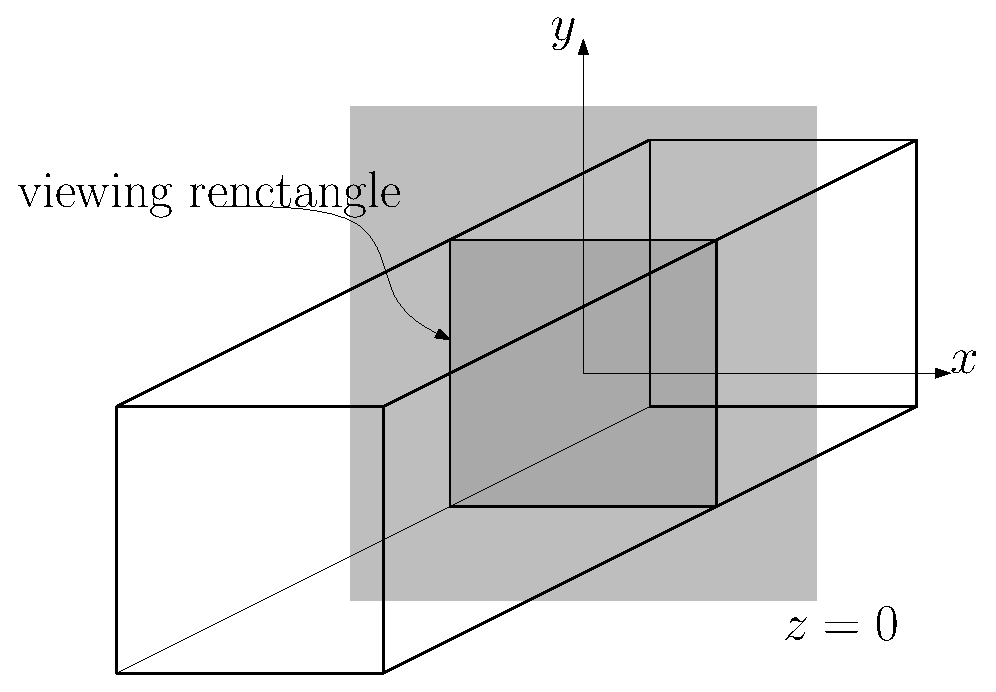
\includegraphics[height=5cm]{OGL_opengl/defaultCam.eps}
    \caption{디폴트 카메라}
    \label{fig:OGL_opengl:defaultCam}
\end{figure}


\subsection{직교 투영(orthographic projection)}

\index{glOrtho}\index{직교 투영}\index{orthographic projection}
디폴트 카메라는 원근이 없는 카메라이다. 이러한 카메라를 직교 투영 카메라라고 한다. 상자 모양의 가시화 공간내의 객체를 상자를 절단하는 면에 투영하는 방식이다. 디폴트 카메라의 경우 중심이 원점이고, 각 변의 길이가 2인 상자 모양인데, 이 위치와 길이를 변경할 수 있다. 이를 지원하는 함수가 glOrtho이며, 이 함수의 원형은 다음과 같다.

\begin{verbatim}
glOrtho(float left, float right, 
        float bottom, float top, 
        float near, float far);
\end{verbatim}

\begin{figure}[h!]
  \centering
    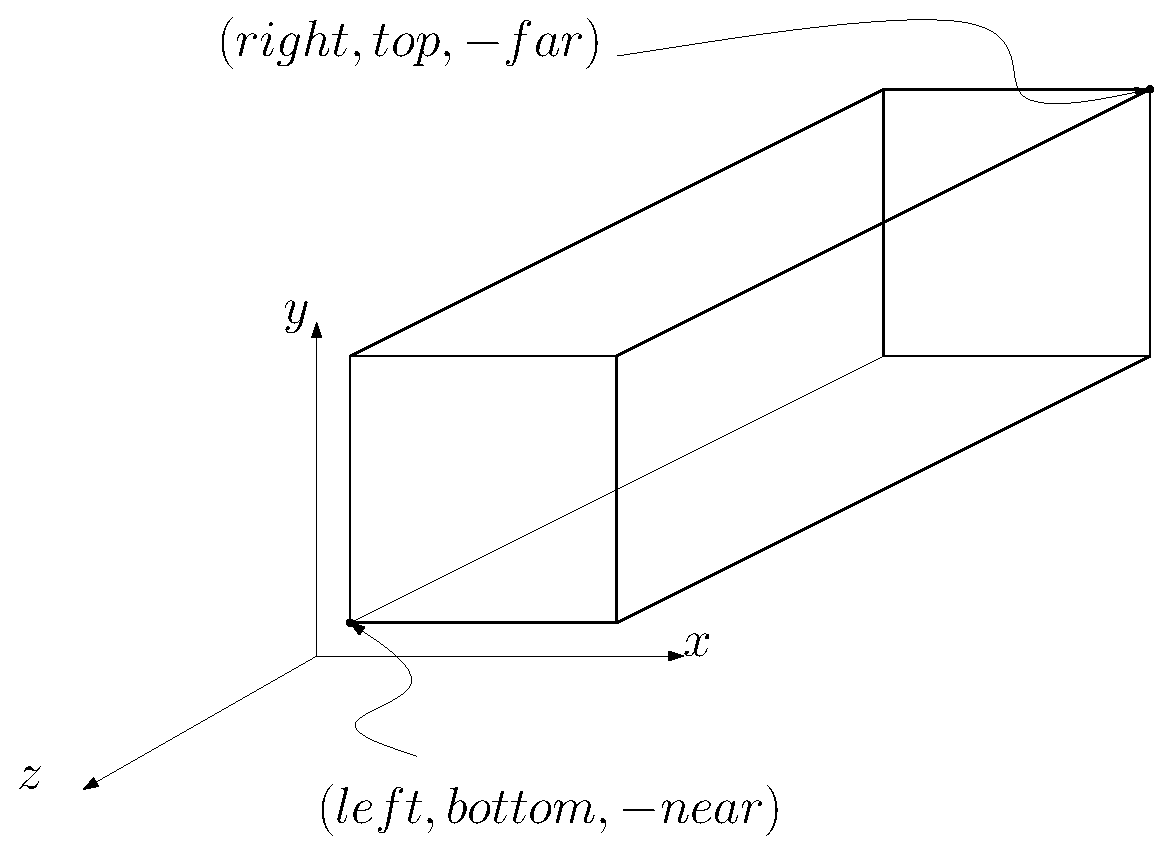
\includegraphics[height=5cm]{OGL_opengl/glOrtho.eps}
    \caption{glOrtho 함수 인자의 의미}
    \label{fig:OGL_opengl:glOrtho}
\end{figure}

각각의 파라미터가 가진 의미는 그림 \ref{fig:OGL_opengl:glOrtho}와 같다. 
여기서 {\sf near}와 {\sf far}의 값에 음수가 적용되어 좌표로 바뀌는 이유는 이 값들이 관찰자로부터의 
거리를 의미하기 때문이다. 이것은 카메라를 다루는 장에서 다시 다룰 것이다.
그림의 파라미터 의미를 고려할 때 결국 OpenGL의 디폴트 카메라는 다음과 같이 설정한 것이다.

\begin{verbatim}
glOrtho(-1,1, -1,1, -1,1);
\end{verbatim}


\subsection{원근 투영 (perspective projection)}

\index{원근 투영}\index{perspective projection}
실제 카메라나 우리 눈은 원근이 없는 평행 투영이 불가능하다. 멀리 있는 것은 작게 보이고 가까이 있는 것은 크게 보이는 이유는 빛이 관측지점으로 모이면서 형성되는 선을 따라 원근투영되기 때문이다. 이러한 원근 투영을 설정하는 방법은 {\sf glFrustum}과 
{\sf gluPerspective}가 있다. {\sf glFrustum}에 대한 이해는 뒤로 미루고 우선 직관적인
{\sf  gluPerspective} 함수를 이해해 보자. 이 함수의 원형은 다음과 같다.

\begin{verbatim}
gluPerspective(float fovy, float Aspect, float near, float far);
\end{verbatim}


{\sf fovy}는 $y$축 방향으로의 시야각을 도(degree)로 나타낸 것이며, {\sf Aspect}는 가시화 볼륨의 종횡비(aspect ratio)를 의미하며, 
{\sf near}는 카메라에서 상이 맺히는 가까운 평면까지의 거리이며, {\sf far}는 가시화가 이루어지는 공간을 결정하는 평면 중 카메라에서 가장 먼 쪽 평면과 카메라 사이의 거리이다.
이 함수는 투영의 속성, 즉 카메라의 렌즈 속성을 결정한다고 생각할 수 있다. 카메라의 렌즈를 바꾸어가면서 관찰하는 것이 아니므로, 이 함수는 그리기 동작이 일어날 때마다 불리는 것이 아니라 초기에 한 번, 혹은 렌즈를 바꿀 필요가 있을 때에만 불리게 된다. 

\subsection{카메라의 위치 변경}

{\sf gluPerspective}를 사용하여도 카메라의 위치는 바뀌지 않는다. 즉 카메라는 여전히 원점 (0,0,0)에 놓여 있는 것이다. 
카메라가 이렇게 고정되어 있으면 사물을 제대로 관찰할 수 없다. 
이 카메라를 원하는 곳으로 옮겨주는 함수가 있는데 바로 {\sf gluLookAt}이다. 이 함수의 원형은 아래와 같다.

\begin{verbatim}
gluLookAt(float eye_x, float eye_y, float eye_z,
          float at_x, float at_y, float at_z,
          float up_x, float up_y, float up_z);
\end{verbatim}


이 함수는 투영의 속성을 바꾸는 것이 아니라 카메라를 옮겨 놓는 것인데, 실제 동작은 카메라 이동의 반대로 물체를 옮겨 놓는 것이다. 이 부분은 다음에 다시 자세히 다루기로 한다. 카메라의 위치는 매 프레임마다 변경될 수 있으므로 이 함수는 그리기 함수 내에서 매번 불리는 것이 일반적이다.


\subsection{행렬 모드(matrix mode)}

\index{행렬 모드} \index{matrix mode}
OpenGL은 세 종류의 행렬을 가지고 있다. 텍스처 행렬, 모델뷰 행렬, 투영행렬이다. 이 가운데 가상공간 내의 좌표를 결정하는 행렬은 모델뷰 행렬과 투영행렬이다. 모델뷰 행렬은 공간 내에서 가상 객체를 변환하여 좌표를 변경하는 데에 사용되는 행렬이며, 투영행렬은 가상 객체를 투영면에 옮겨 놓는 데에 사용되는 행렬이다. OpenGL이 그리는 모든 객체의 좌표는 우선 모델뷰 행렬에 곱해져서 자리를 잡고, 투영행렬이 곱해져서 평면에 놓이게 되는 것이다. 

\begin{algorithmbis}[카메라 특성과 위치 설정의 예]\label{code:OGL_opengl:camSetting}
\lstset{language=C++, escapechar=^} 
\begin{lstlisting}
glMatrixMode(GL_PROJECTION);
glLoadIdentity();
gluPerspective(60, 1.0, 0.1, 100.0);

glMatrixMode(GL_MODELVIEW);
glLoadIdentity();
gluLookAt(1.0, 1.0, 1.0, 0.0, 0.0, 0.0, 0.0, 1.0, 0.0);

^{\sf [[draw something]]}^
\end{lstlisting}
\end{algorithmbis}

이 두 행렬은 나중에 다시 깊이 살펴볼 것이다. 여기서는 {\sf gluPerspective}와 {\sf gluLookAt}이 어떠한 행렬 모드을 변경하는가 하는 것이 관심이다. {\sf gluPerspective} 함수는 투영의 특성을 변경하는 것이므로 투영행렬 모드에서 동작한다. 반면 {\sf gluLookAt}은 투영의 특성이 아니라 카메라의 위치를 옮기는 것이고, 이는 바꾸어 말해 물체의 위치를 카메라 기준에서 옮기는 것이므로 모델뷰 행렬을 변경하는 것이다. 따라서 이 함수들은 각각 적절한 행렬 모드에서 동작해야 하며 코드 \ref{code:OGL_opengl:camSetting}와 같은 방식으로 프로그램에 포함된다. 이러한 코드를 이용하여 카메라를 재배치하는 프로그램을 작성할 수 있다. 코드 \ref{code:OGL_opengl:SceneWithCam}는 그러한 예이다.

\begin{algorithmbis}[카메라를 설정하는 기본적인 프로그램]\label{code:OGL_opengl:SceneWithCam}
\lstset{language=C++, escapechar=^} 
\begin{lstlisting}
^{\sf [[header 파일 포함하기...]]}^

void init(int argc, char **argv) {
  // ^{\it 윈도우 생성, 버퍼 설정}^
  glutInit(&argc, argv);
  glutInitDisplayMode(GLUT_SINGLE|GLUT_RGBA);
  glutInitWindowPosition(0,0);
  glutInitWindowSize(512,512);
  glutCreateWindow("Dr. Kang's Graphics Lecture");
  glClearColor(1.0, 1.0, 1.0, 1.0);
  // ^{\it 카메라 투영 특성 설정 (glPerspective 사용). 이때는 GL\_PROJECTION 행렬모드여야 한다.}^
  glMatrixMode(GL_PROJECTION);
  glLoadIdentity();
  gluPerspective(60, 1.0, 0.1, 100.0);
}

void drawScene() {
  ^{\sf [[앞서 사용한 코드 \ref{code:OGL_opengl:simpleScene}의 그리기 코드를 여기에 넣는다. (단, glFlush는 여기서 사용하지 않는다)]]}^
}
void drawAxes() {
  glBegin(GL_LINES);
  glColor3f(1.0, 0.0, 0.0);
  glVertex3f(0.0, 0.0, 0.0);   glVertex3f(1.0, 0.0, 0.0);
  glColor3f(0.0, 1.0, 0.0);
  glVertex3f(0.0, 0.0, 0.0);  glVertex3f(0.0, 1.0, 0.0);
  glColor3f(0.0, 0.0, 1.0);
  glVertex3f(0.0, 0.0, 0.0);  glVertex3f(0.0, 0.0, 1.0);
  glEnd();
}

void display() {
  static float t=0.0;
  // ^{\it 카메라의 위치와 방향을 설정한다. 이때는 GL\_MODELVIEW 행렬 모드여야 한다.}^
  glMatrixMode(GL_MODELVIEW);
  glLoadIdentity();
  gluLookAt( 2.0*sin(t), 1, 2.0*cos(t), 0, 0, 0,  0, 1, 0);
  t+=0.001;
  glClear(GL_COLOR_BUFFER_BIT);
  drawScene();		
  glLineWidth(5);
  drawAxes();		
  glLineWidth(1);
  glFlush();
};

int main (int argc, char **argv) {
  init(argc, argv);
  glutDisplayFunc(display);
  glutIdleFunc(display);
  glutMainLoop();
}
\end{lstlisting}
\end{algorithmbis}

코드. \ref{code:OGL_opengl:SceneWithCam}를 통해 얻을 수 있는 결과는 그림. \ref{fig:OGL_opengl:camMove}를 통해 확인할 수 있다.
이 코드를 실행하면 앞서 그렸던 평면적인 장면이 3차원 공간에서 입체적으로 회전하는 모습을 볼 수 있다.
코드의 의미를 해석하자면, $xz$ 평면에서 원점을 중심으로 반지름 2.0인 원의 원주 위에 카메라를 두고 원주를 따라 돌면서
쳐다보는 방향은 원점으로 고정한 것이다. 공간을 좀 더 잘 확인할 수 있도록 세 개의 축을 그려 넣었다.

\begin{figure}[h!]
  \centering
    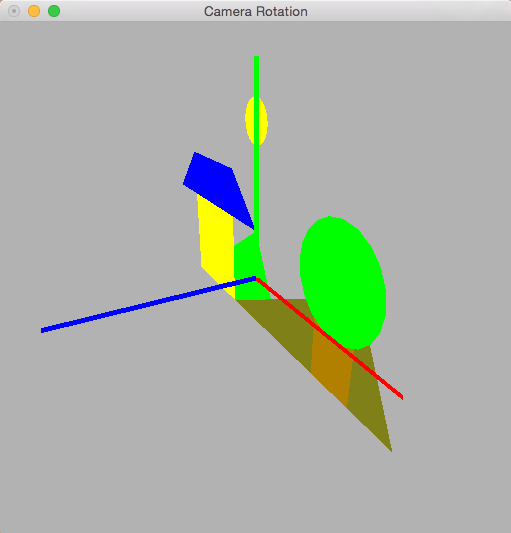
\includegraphics[height=10cm]{OGL_opengl/camMove.png}
    \caption{카메라의 위치와 방향이 변경된 결과}
    \label{fig:OGL_opengl:camMove}
\end{figure}

\section{입체와 깊이 버퍼의 활용}

앞 절에서 카메라를 옮겨 보았다. 이를 통해 우리가 그리고 보는 공간이 3차원 공간임을 확인할 수 있었다. 그러나, 아직은 납작한 평면에 그림을 그리고 돌려본 상태이다. 부피를 가진 입체 도형을 그리는 것이 이 절의 주제이다.
좌표를 3차원으로 설정하면 입체는 그려진다. 2차원 그리기와 전혀 다를 바가 없는 문제이다. 그러나 여기에서 우리는 새로운 문제를 만나게 된다.
다음의 크드. \ref{code:OGL_opengl:3DObjects}와 같은 그리기 코드가 있다. {\sf display} 함수에서 
이 코드에 나타나 있는 {\sf draw} 함수를 호출하면 어떤 그림이 그려질지 상상해 보자.


이 그리기 코드는 노란색 뚜껑과, 하늘색 바닥이 있고, 왼쪽에는 초록색 벽, 오른쪽에는 흰색 벽을 그리고, 입체 안에 3 개의 축을 그리는 코드이다. 그런데 앞서 작성된 코드의 {\sf display} 콜백 함수 내에 {\sf draw()}를 삽입하면 그림. \ref{fig:OGL_opengl:noZBuff}와 같이 그려진다.
지정한 좌표에 제대로 그려진 것 같지만 자세히 살펴보면 무엇인가 이상하다.

\begin{algorithmbis}[입체 도형 그리기 예제]\label{code:OGL_opengl:3DObjects}
\lstset{language=C++, escapechar=^} 
\begin{lstlisting}
void drawScene() {
  // drawing code
  glBegin(GL_QUADS);
  // ^{\it 천정}^
  glColor3f(1.0, 1.0, 0.0);
  glVertex3f(-0.5, 0.5, -0.5);
  glVertex3f( 0.5, 0.5, -0.5);
  glVertex3f( 0.5, 0.5,  0.5);
  glVertex3f(-0.5, 0.5,  0.5);
  // ^{\it 바닥}^
  glColor3f(0.0,1.0,1.0);
  glVertex3f(-0.5,-0.5, -0.5);
  glVertex3f( 0.5,-0.5, -0.5);
  glVertex3f( 0.5,-0.5,  0.5);
  glVertex3f(-0.5,-0.5,  0.5);
  // ^{\it 왼쪽 벽}^
  glColor3f(0.0,1.0,0.0);
  glVertex3f(-0.5, 0.5, -0.5);
  glVertex3f(-0.5, 0.5,  0.5);
  glVertex3f(-0.5,-0.5,  0.5);
  glVertex3f(-0.5,-0.5, -0.5);
  // ^{\it 오른쪽 벽}^
  glColor3f(1.0,1.0,1.0);
  glVertex3f( 0.5, 0.5, -0.5);
  glVertex3f( 0.5, 0.5,  0.5);
  glVertex3f( 0.5,-0.5,  0.5);
  glVertex3f( 0.5,-0.5, -0.5);
  glEnd();
}

void draw() {
  drawScene();
  drawAxes(); //^{\it drawAxes 함수는 코드 \ref{code:OGL_opengl:SceneWithCam}에서 사용한 것을 그대로 쓴다.}^
}
\end{lstlisting}
\end{algorithmbis}


\begin{figure}[h!]
  \centering
    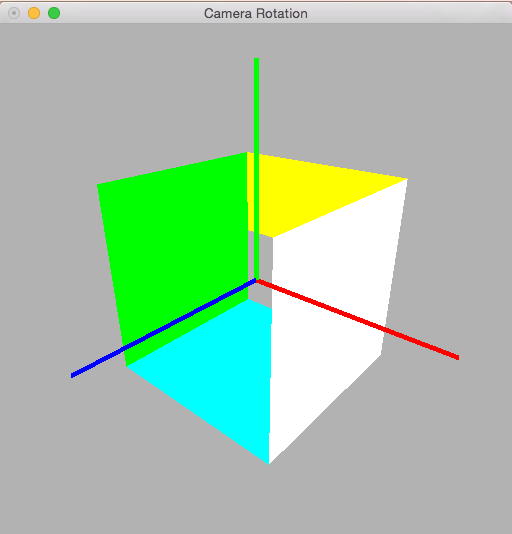
\includegraphics[height=10cm]{OGL_opengl/noZBuff.png}
    \caption{입체의 깊이가 고려되지 않은 결과}
    \label{fig:OGL_opengl:noZBuff}
\end{figure}

노란색 뚜겅이 뒤에 있는 초록색 벽에 가려지는 현상이 발생하며, 벽이나 뚜껑에 의해 일부가 가려져야 하는 축이 전혀 가려지지 않고 그려지고 있다.
이 문제는 OpenGL에게 그려지는 픽셀의 깊이를 고려하도록 하지 않을 경우에 발생하는 문제이다.
OpenGL에게 그려진 픽셀의 깊이를 고려하라고 하지 않았기 때문에 지금 그리려고 하는 객체의 픽셀이 
이미 그려진 객체에 가려지는지를 검사하지 않는 것이다.
이럴 경우 가장 나중에 그려진 것은 다른 객체와의 깊이를 따지지 않고 무조건 화면에 나타나게 된다.
예를 들어 이 코드에서는 축이 가장 나중에 그려졌기 때문에 어느 누구에게도 가려지지 않는다.
이러한 문제는 깊이 버퍼를 사용하여 해결할 수 있다.

\subsection{깊이 버퍼(depth buffer)의 사용}

\index{z-buffer}\index{color buffer}
\index{z-버퍼}\index{색상 버퍼}
z-버퍼라고도 불리는 깊이 버퍼는 영상을 생성할 때에 사용되는 여러 버퍼 가운데 하나이다. 가장 일반적인 버퍼는 색상 버퍼(color buffer)인데, 그려지는 영상의 각 화소별 색을 기록하는 것이다. 우리가 최종적으로 보게되는 것은 이 색상 버퍼의 내용이 된다. 그런데, 이런 색상 버퍼를 구성할 때 물체의 가려짐을 고려하여 가려진 물체를 그리지 않도록 해야 하는데, 이를 해결하는 버퍼가 깊이 버퍼이다. 깊이 버퍼는 객체를 그릴 때, 색상이 아니라 카메라에서 그려지는 픽셀까지의 거리를 저장하는 버퍼이다. 그림. \ref{fig:OGL_opengl:Z_Buffer}는 그래픽스 프로그램에서 일반적으로 가시화되는 색상 버퍼의 내용과, 이 장면에 해당하는 깊이 버퍼를 비교하고 있다.

\begin{figure}[h!]
  \centering
    \includegraphics[height=10cm]{OGL_opengl/Z_Buffer.png}
    \caption{가시화되는 색샹 버퍼의 내용과 객체의 깊이 정보를 담은 z-버퍼의 비교}
    \label{fig:OGL_opengl:Z_Buffer}
\end{figure}


깊이 버퍼가 있다면 어떤 픽셀을 그릴 때에 이미 그려진 픽셀의 깊이를 보고 이 깊이 값보다 새로 그리려는 픽셀의 깊이값이 카메라에서 가까운 값일 경우에만 그림을 그린다. 이 방법은 일반적으로 하드웨어를 통해 이루어진다.
깊이 버퍼를 사용함으로써 우리는 효율적으로 가려져서 보이지 않는 물체를 렌더링에서 제외시킬 수 있다. 
OpenGL에서는 이러한 깊이 버퍼를 쉽게 사용할 수 있도록 지원한다. GLUT 라이브러리를 사용한다고 가정하면 {\sf glutInitDisplayMode} 함수를 이용하여 다음과 같이 설정하면 깊이 버퍼를 사용할 수 있다.

\begin{itemize}
\item{\sf glutInitDisplayMode(GLUT\_SINGLE $|$ \color{red}{GLUT\_DEPTH} $|$ GLUT\_RGBA);}
\end{itemize}

\index{GL\_DEPTH\_TEST}
하지만 이렇게 깊이 버퍼를 사용한다고 해서 깊이 버퍼를 활용하여 가려진 물체를 렌더링에서 제외하는 작업이 이루어지지는 않는다. OpenGL은 기본적으로 깊이를 검사하는 “깊이 테스트” 작업을 수행하지 않는 것이 디폴트 상태이기 때문이다. 깊이 테스트를 수행하기 위해서는 다음과 같이 상태를 변경해야 한다.

\begin{itemize}
\item{\sf glEnable(\color{red}{GL\_DEPTH\_TEST});}
\end{itemize}

또한 매번 그리기가 이뤄지면 그려진 내용에 따라 깊이 버퍼의 내용이 더러워져 있는 상태가 되므로, 새로운 그리기를 하기 전에 색상 버퍼를 깨끗하게 지우듯이 깊이 버퍼의 내용도 깨끗하게 지우는 다음과 같은 코드가 필요하다.

\index{GL\_DEPTH\_BUFFER\_BIT}
\begin{itemize}
\item{\sf glClear( GL\_COLOR\_BUFFER\_BIT $|$ \color{red}{GL\_DEPTH\_BUFFER\_BIT});}
\end{itemize}
이상과 같이 깊이 버퍼의 설정과 깊이 테스트를 수행하도록 상태를 변경하면 앞서의 결과는 다음과 같이 기대했던 것과 같이 그려지게 된다.
그림에서 축은 자연스럽게 뚜겅과 우측 벽에 의해 가려지고 있으며, 좌측 벽도 뚜껑에 가려져 나타나게 된다.


\subsection{이중 버퍼의 사용}

\index{이중 버퍼}\index{double buffering}
우리는 지금까지 색상과 깊이 버퍼가 하나만 존재하는 단일 버퍼 환경에서 작업을 하였다. 그런데 이러한 단일 버퍼 환경은 애니메이션 등이 있을 때 하나의 버퍼를 다 지우고 새로운 그림을 그리는 과정에서 화면 깜빡임이 있을 수 있다.
화면 깜빡임을 해결하는 방법은 버퍼를 앞 버퍼(front buffer)와 뒷 버퍼(back buffer)의 이중 구조로 만들어 앞 버퍼가 출력되고 있을 때 다음에 보여질 그림은 뒷 버퍼에 그리는 것이다. 그리고 뒷 버퍼의 그림이 다 그려지고 화면에 보여질 준비가 마쳤을 때, 앞 버퍼와 뒷 버퍼의 역할을 뒤바꾸는 버퍼 스와핑(swaping)을 수행하는 것이다. 지금부터 본 자료의 모든 코드는 이러한 이중 버퍼의 사용을 기본으로 하겠다. 

\index{GL\_SINGLE}\index{GL\_DOUBLE}
이중 버퍼를 실제로 사용하는 방법은 다음과 같이 우선 glutInitDisplayMode 함수에서 {\sf GL\_SINGLE}을 {\sf GL\_DOUBLE}로 바꾸어 시스템이 두 개의 버퍼를 준비하게 하는 것이다.

\begin{itemize}
\item {\sf glutInitDisplayMode( \color{red}{GLUT\_DOUBLE} $|$ GLUT\_DEPTH $|$ GLUT\_RGBA);}
\end{itemize}

\index{glutSwapBuffers}
또한 버퍼의 송출은 {\sf glFlush}가 아니라 {\sf glutSwapBuffers}를 이용한다.

\begin{itemize}
\item {\sf glutSwapBuffers();}
\end{itemize}

이상과 같은 방법을 통해 화면의 깜박임이 업는 이중 버퍼링 활용이 가능하다. 지금까지의 내용을 정리하여 소스코드는 다음 코드. \ref{code:OGL_opengl:3DObjectsWithZbuff}와 같이 애니메이션 되는 이중버퍼-깊이버퍼 사용 예제 코드로 개선이 가능하다.

이때 {\sf keyboard}라는 함수가 추가로 구현되었고, 이를 {\sf glutKeyboardFunc}를 이용하여 키보드 처리 콜백 함수로 사용하고 있다. 이 내용은 쉽게 이해할 수 있으므로 설명을 생략한다. 다만 이 함수 안에 있는 {\sf glutPostRedisplay} 함수에 대한 설명이 필요한데, 이 함수는 사용자가 강제로 그리기 이벤트를 발생 시키는 것이다. 즉 키보드 입력이 있으면 자동으로 그려지기가 불리게 된다.

\begin{algorithmbis}[애니메이션이 포함된 깊이버퍼/이중버퍼 활용 예제]\label{code:OGL_opengl:3DObjectsWithZbuff}
\lstset{language=C++, escapechar=^} 
\begin{lstlisting}

^{\sf [[헤더 파일 포함하기]]}^

void init(int argc, char **argv) {
    // ^{\it 윈도우 생성, 버퍼 설정}^
    glutInit(&argc, argv);
    // ^{\it 이중 버퍼링, RGBA 색상 버퍼와 함께, 깊이 버퍼를 준비하도록 한다.}^
    glutInitDisplayMode(GLUT_DOUBLE|GLUT_RGBA|GLUT_DEPTH);
    glutInitWindowPosition(0,0);
    glutInitWindowSize(512,512);
    glutCreateWindow("DEPTH BUFFER");
    glClearColor(0.7, 0.7, 0.7, 1.0);
    // ^{\it 깊이 버퍼 검사를 활성화한다.}^
    glEnable(GL_DEPTH_TEST);
    // ^{\it 카메라 투영 특성 설정 (glPerspective 사용). 이때는 GL\_PROJECTION 행렬모드여야 한다.}^
    glMatrixMode(GL_PROJECTION);
    glLoadIdentity();
    gluPerspective(60, 1.0, 0.1, 100.0);
}
void drawScene() {     ^{\sf [[코드 \ref{code:OGL_opengl:3DObjects}와 동일]]}^  }
void drawAxes() {     ^{\sf [[코드 \ref{code:OGL_opengl:3DObjects}와 동일]]}^ }
void draw() { ^{\sf [[코드 \ref{code:OGL_opengl:3DObjects}와 동일]]}^  }
void display() {
    static float t=0.0;
    // ^{\it 카메라의 위치와 방향을 설정한다. 이때는 GL\_MODELVIEW 행렬 모드여야 한다.}^
    glMatrixMode(GL_MODELVIEW);
    glLoadIdentity();
    gluLookAt( 2.0*sin(t), 1, 2.0*cos(t), 0, 0, 0,  0, 1, 0);
    t+=0.001;
    // ^{\it 컬러 버퍼 뿐만 아니라 깊이 버퍼도 매 프레임마다 지운다.}^
    glClear(GL_COLOR_BUFFER_BIT|GL_DEPTH_BUFFER_BIT);
    draw();
    glutSwapBuffers();
};
\end{lstlisting}
\end{algorithmbis}

이상의 코드를 수행하면, 그림. \ref{fig:OGL_opengl:ZBuff}와 같이 3차원 공간에서 각각의 객체가 시점으로부터 얼마나 떨어져 있는지를 비교하여 뒤에 있는 물체가 앞의 물체에 의해 가려지는 효과를 잘 표현할 수 있다.

\begin{figure}[h!]
  \centering
    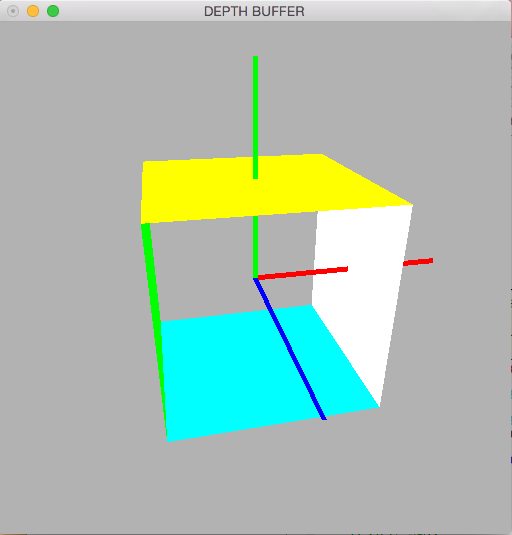
\includegraphics[height=10cm]{OGL_opengl/ZBuff.png}
    \caption{z-버퍼를 이용한 객체의 깊이 비교 적용 결과}
    \label{fig:OGL_opengl:ZBuff}
\end{figure}
 
OpenGL에 대한 소개는 \cite{woo1999openGL,wright2004openGL} 등을 참고하라.


